\begin{figure}[H]
\centering
\begin{minipage}[t]{0.48\textwidth}
\centering
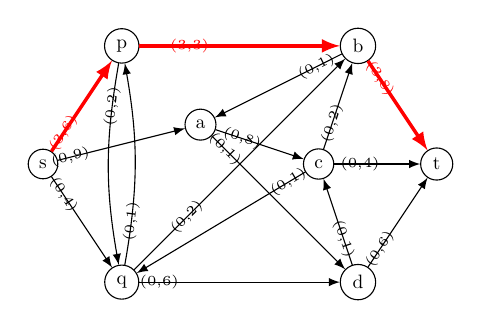
\begin{tikzpicture}
	\node (s) at (-1,1.5) [circle,draw, fill = white, scale = 0.7] {s};
	\node (q) at (0,0) [circle,draw, fill = white, scale = 0.7] {q};
	\node (d) at (3,0) [circle,draw, fill = white, scale = 0.7] {d};
	\node (t) at (4,1.5) [circle,draw, fill = white, scale = 0.7] {t};
	\node (b) at (3,3) [circle,draw, fill = white, scale = 0.7] {b};
	\node (p) at (0,3) [circle,draw, fill = white, scale = 0.7] {p};
	\node (a) at (1,2) [circle,draw, fill = white, scale = 0.7] {a};
	\node (c) at (2.5,1.5) [circle,draw, fill = white, scale = 0.7] {c};
	\draw[-latex] (a) -- (c) node [pos = 0.3, sloped] {\tiny(0,8)};
	\draw[-latex] (a) -- (d) node [pos = 0.1, sloped] {\tiny(0,1)};
	\draw[-latex] (b) -- (a) node [pos = 0.2, sloped] {\tiny(0,1)};
	\draw[-latex,line width=1.25,red] (b) -- (t) node [pos = 0.2, sloped] {\tiny(3,8)};
	\draw[-latex] (c) -- (b) node [pos = 0.3, sloped] {\tiny(0,2)};
	\draw[-latex] (c) -- (q) node [pos = 0.1, sloped] {\tiny(0,1)};
	\draw[-latex] (c) -- (t) node [pos = 0.3, sloped] {\tiny(0,4)};
	\draw[-latex] (d) -- (c) node [pos = 0.3, sloped] {\tiny(0,1)};
	\draw[-latex] (d) -- (t) node [pos = 0.2, sloped] {\tiny(0,6)};
	\draw[-latex,line width=1.25,red] (p) -- (b) node [pos = 0.25, sloped] {\tiny(3,3)};
	\draw[-latex] (p) to [bend right=10] node [pos = 0.2, sloped] {\tiny(0,2)} (q);
	\draw[-latex] (q) to [bend right=10] node [pos = 0.2, sloped] {\tiny(0,1)} (p);
	\draw[-latex] (q) -- (b) node [pos = 0.25, sloped] {\tiny(0,2)};
	\draw[-latex] (q) -- (d) node [pos = 0.1, sloped] {\tiny(0,6)};
	\draw[-latex] (s) -- (q) node [pos = 0.2, sloped] {\tiny(0,4)};
	\draw[-latex,line width=1.25,red] (s) -- (p) node [pos = 0.2, sloped] {\tiny(3,6)};
	\draw[-latex] (s) -- (a) node [pos = 0.1, sloped] {\tiny(0,9)};
\end{tikzpicture}
\caption{}\label{fig:spbt}
\end{minipage}% fig:spbt
\begin{minipage}[t]{0.48\textwidth}
\centering
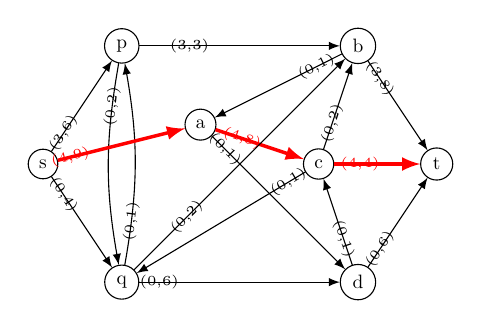
\begin{tikzpicture}
	\node (s) at (-1,1.5) [circle,draw, fill = white, scale = 0.7] {s};
	\node (q) at (0,0) [circle,draw, fill = white, scale = 0.7] {q};
	\node (d) at (3,0) [circle,draw, fill = white, scale = 0.7] {d};
	\node (t) at (4,1.5) [circle,draw, fill = white, scale = 0.7] {t};
	\node (b) at (3,3) [circle,draw, fill = white, scale = 0.7] {b};
	\node (p) at (0,3) [circle,draw, fill = white, scale = 0.7] {p};
	\node (a) at (1,2) [circle,draw, fill = white, scale = 0.7] {a};
	\node (c) at (2.5,1.5) [circle,draw, fill = white, scale = 0.7] {c};
	\draw[-latex,line width=1.25,red] (a) -- (c) node [pos = 0.3, sloped] {\tiny(4,8)};
	\draw[-latex] (a) -- (d) node [pos = 0.1, sloped] {\tiny(0,1)};
	\draw[-latex] (b) -- (a) node [pos = 0.2, sloped] {\tiny(0,1)};
	\draw[-latex] (b) -- (t) node [pos = 0.2, sloped] {\tiny(3,8)};
	\draw[-latex] (c) -- (b) node [pos = 0.3, sloped] {\tiny(0,2)};
	\draw[-latex] (c) -- (q) node [pos = 0.1, sloped] {\tiny(0,1)};
	\draw[-latex,line width=1.25,red] (c) -- (t) node [pos = 0.3, sloped] {\tiny(4,4)};
	\draw[-latex] (d) -- (t) node [pos = 0.2, sloped] {\tiny(0,6)};
	\draw[-latex] (d) -- (c) node [pos = 0.3, sloped] {\tiny(0,1)};
	\draw[-latex] (p) -- (b) node [pos = 0.25, sloped] {\tiny(3,3)};
	\draw[-latex] (p) to [bend right=10] node [pos = 0.2, sloped] {\tiny(0,2)} (q);
	\draw[-latex] (q) to [bend right=10] node [pos = 0.2, sloped] {\tiny(0,1)} (p);
	\draw[-latex] (q) -- (b) node [pos = 0.25, sloped] {\tiny(0,2)};
	\draw[-latex] (q) -- (d) node [pos = 0.1, sloped] {\tiny(0,6)};
	\draw[-latex] (s) -- (q) node [pos = 0.2, sloped] {\tiny(0,4)};
	\draw[-latex] (s) -- (p) node [pos = 0.2, sloped] {\tiny(3,6)};
	\draw[-latex,line width=1.25,red] (s) -- (a) node [pos = 0.1, sloped] {\tiny(4,9)};
\end{tikzpicture}
\caption{}\label{fig:sact}
\end{minipage}% fig:sact
\end{figure}% 1st row

 \begin{pspicture}(5,5)
   %% Triangle in red:
   \pspolygon[linecolor=red](1,1)(5,1)(1,4)
   %% Bezier curve in green:
   \pscurve[linecolor=green,linewidth=2pt,%
     showpoints=true](5,5)(3,2)(4,4)(2,3)
   %% Circle in blue with radius 1:
   \pscircle[linecolor=blue,linestyle=dashed](3,2.5){1}
 \end{pspicture}

  \begin{pspicture*}(-7,-2)(7,2)
   \psaxes[labels=none](0,0)(-7,-2)(7,2)        % sets up axis
   \psplot[linecolor=blue, linewidth=1.5pt]%    % plots the sinewave
     {-7}{7}{x 0.01745329252 div sin}           % notice the RPN expression
   \uput[45](3.1415926,0){$\pi$}                % these are the labels
   \uput[90](-1.570796,0){$-\pi/2$}             % \uput is a box positioned at [angle]
   \uput[-90](1.570796,0){$\pi/2$}              % relative to (x,y) coordinate
   \uput[-135](-3.1415926,0){$-\pi$}            % and putting { content } on the box
   \psline[linewidth=1pt,linecolor=red,linestyle=dotted]%   % red dotted lines
     (1.57079632,1)(1.57079632,0)
   \psline[linewidth=1pt,linecolor=red,linestyle=dotted]%
     (-1.57079632,-1)(-1.57079632,0)
 \end{pspicture*}






